\documentclass[12pt]{extarticle}
%Some packages I commonly use.
\usepackage[portuguese]{babel}
\usepackage{graphicx}
\usepackage{framed}
\usepackage[normalem]{ulem}
\usepackage{amsmath}
\usepackage{amsthm}
\usepackage{amssymb}
\usepackage{amsfonts}
\usepackage{enumerate}
\usepackage[utf8]{inputenc}
\usepackage{float}
\usepackage{gensymb}
\usepackage[top=1 in,bottom=1in, left=1 in, right=1 in]{geometry}
\usepackage{multirow}
\usepackage{caption}
\usepackage{subcaption}
\usepackage[utf8]{inputenc}

%A bunch of definitions that make my life easier
\newcommand{\matlab}{{\sc Matlab} }
\newcommand{\cvec}[1]{{\mathbf #1}}
\newcommand{\rvec}[1]{\vec{\mathbf #1}}
\newcommand{\ihat}{\hat{\textbf{\i}}}
\newcommand{\jhat}{\hat{\textbf{\j}}}
\newcommand{\khat}{\hat{\textbf{k}}}
\newcommand{\minor}{{\rm minor}}
\newcommand{\trace}{{\rm trace}}
\newcommand{\spn}{{\rm Span}}
\newcommand{\rem}{{\rm rem}}
\newcommand{\ran}{{\rm range}}
\newcommand{\range}{{\rm range}}
\newcommand{\mdiv}{{\rm div}}
\newcommand{\proj}{{\rm proj}}
\newcommand{\R}{\mathbb{R}}
\newcommand{\N}{\mathbb{N}}
\newcommand{\Q}{\mathbb{Q}}
\newcommand{\Z}{\mathbb{Z}}
\newcommand{\<}{\langle}
\renewcommand{\>}{\rangle}
\renewcommand{\emptyset}{\varnothing}
\newcommand{\attn}[1]{\textbf{#1}}
\theoremstyle{definition}
\newtheorem{theorem}{Theorem}
\newtheorem{corollary}{Corollary}
\newtheorem*{definition}{Definition}
\newtheorem*{example}{Example}
\newtheorem*{note}{Note}
\newtheorem{exercise}{Exercise}
\newcommand{\bproof}{\bigskip {\bf Proof. }}
\newcommand{\eproof}{\hfill\qedsymbol}
\newcommand{\Disp}{\displaystyle}
\newcommand{\qe}{\hfill\(\bigtriangledown\)}
\setlength{\columnseprule}{1 pt}
\usepackage[utf8]{inputenc}

\title{Introdução à ondulatória}
\author{Felipe Salvador}
\date{Atualizado em \today}

\begin{document}

\maketitle

\section{Introdução}
A ondulatória é a área da física responsável pelo estudo de \textbf{ondas}. \textbf{Ondas são pertubações num objeto/meio que transporta energia de um ponto ao outro.} Uma característica especial das ondas é que a propagação de ondas não involve transporte de matéria, ou seja, átomos dos meios não se movimentam durante a passagem da onda.

O nome que damos à pertubação gerada no meio é \textbf{pulso} e um pulso constitui uma \textbf{onda}. Se a pertubação acontecer várias vezes seguidas, teremos uma sequências de pulsos que constitui \textbf{uma frente de onda ou trem de onda.}

\section{Tipos de Ondas}
Nós podemos categorizar as ondas de 3 formas de diferentes: \textbf{pela forma de vibração da onda, pela direção de propagação ou pela natureza da onda.}

\subsection{Forma de vibração}
Há 2 tipos de onda nessa categorização:
\begin{itemize}
    \item \textbf{Ondas longitudinais} - ondas em que a vibração acontece numa direção paralela à direção de propagação da onda;
    \item \textbf{Ondas transversais} - ondas em que a vibração acontece numa direção perpendicular à direção de propagação da onda.
\end{itemize}
\begin{figure}[H]
    \centering
    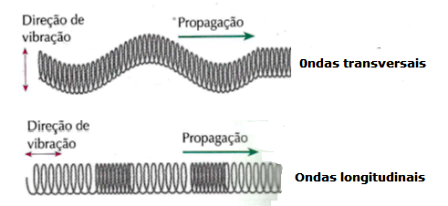
\includegraphics[width=0.55\textwidth]{ondas_longitudinais_transversais.png}
    \caption{Diagrama das ondas longitudinais e transversais.}
    \label{fig:longitudinal_transversal}
\end{figure}

\textbf{Exemplo de onda longitudinal é a onda de som. Exemplo de transversal é a onda luminosa.}

\subsection{Direção de propação}
Há 3 tipos de onda nessa categoria:
\begin{itemize}
    \item \textbf{Ondas unidimensionais} - são ondas que se propagam numa única direção;
    \item \textbf{Ondas bidimensionais ou circulares} - são ondas que se propagam num plano (2 direções);
    \item \textbf{Ondas tridimensionais ou esféricas} - são ondas que se propagam no espaço (3 direções)
\end{itemize}

\begin{figure}[H]
     \centering
     \begin{subfigure}[b]{0.3\textwidth}
         \centering
         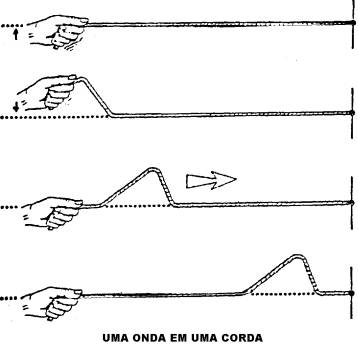
\includegraphics[width=\textwidth]{unidimensionais.jpg}
         \caption{Diagrama de onda unidimensional - ondas numa corda}
         \label{fig:unidimensional}
     \end{subfigure}
     \hfill
     \begin{subfigure}[b]{0.3\textwidth}
         \centering
         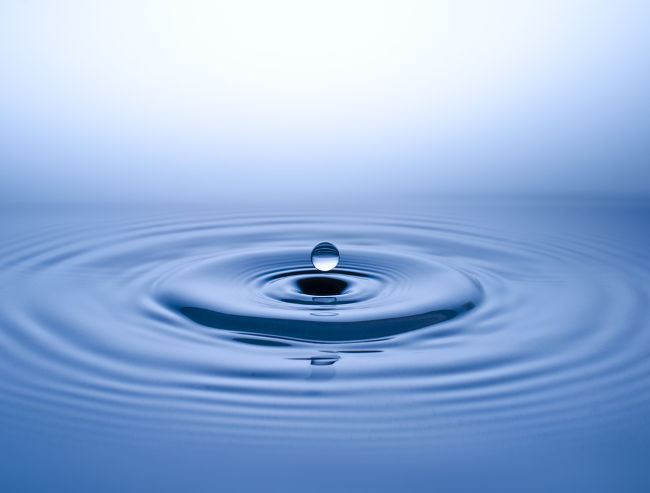
\includegraphics[width=\textwidth]{bidimensionais.jpg}
         \caption{Diagrama de onda bidimensional - ondas na superfície da água}
         \label{fig:bidimensional}
     \end{subfigure}
     \hfill
     \begin{subfigure}[b]{0.3\textwidth}
         \centering
         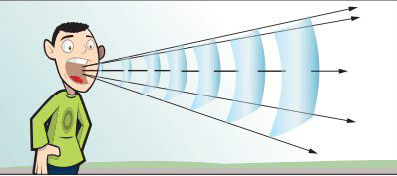
\includegraphics[width=\textwidth]{tridimensionais.png}
         \caption{Diagrama de onda tridimensional - ondas de som geradas pelas cordas vocais}
         \label{fig:tridimensionais}
     \end{subfigure}
        \caption{Exemplos de ondas uni,bi e tridimensionais}
        \label{fig:ondas_propagacao}
\end{figure}

\subsection{Natureza da Onda}
Há 2 tipos de onda nessa categoria:
\begin{itemize}
    \item \textbf{Ondas mecânicas} - ondas que são geradas de modo mecânico por meio de deformação elástica ou compressão. \textbf{Ondas mecânicas se propagam somente em meios materiais (ar, água, vidro, metais).}
    \item \textbf{Ondas eletromagnéticas} - ondas que são geradas por meio da oscilação ou aceleração de cargas elétricas. \textbf{As ondas eletromagnéticas são ondas que não precisam de meios materiais para se propagar (podem se propagar no vácuo) e são ondas transversais.}
\end{itemize}

\begin{figure}[H]
     \centering
     \begin{subfigure}[b]{0.45\textwidth}
         \centering
         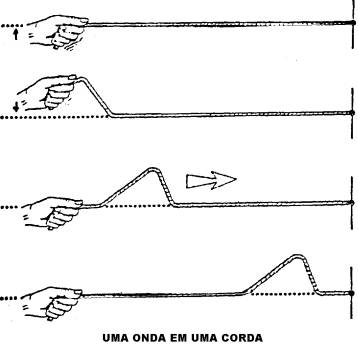
\includegraphics[width=\textwidth]{unidimensionais.jpg}
         \caption{Diagrama de onda mecânica - onda numa corda}
         \label{fig:mecanica}
     \end{subfigure}
     \hfill
     \begin{subfigure}[b]{0.45\textwidth}
         \centering
         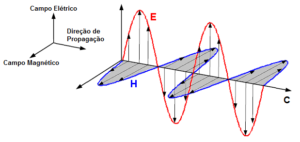
\includegraphics[width=\textwidth]{ondas_eletro.png}
         \caption{Diagrama de onda eletromagnética - onda luminosa}
         \label{fig:eletromagnetica}
     \end{subfigure}
        \caption{Exemplos de ondas mecânicas e eletromagnéticas}
        \label{fig:ondas_natureza}
\end{figure}

\section{Propagação de ondas em 1D}

Nós só iremos nos reter a estudar ondas mecânicas que se propagam numa única direção. Para isso, considere uma corda de um material homogêneo (a sua massa é distribuida igualmente por toda extensão). Também vamos considerar que a corda é uma fio perfeito, ou seja, não altera o formato do pulso/onda que é propagado nela.

Dito isso, a velocidade de propagação da onda na corda é definida como:
\begin{equation}
    v = \sqrt{\frac{F_T}{\mu_L}}
\end{equation}
\noindent em que '$F_T$' é a força de tração aplicada nas extremidades das ondas e '$\mu_L = \frac{m}{L}$' é a densidade linear de massa (razão entre a massa da corda por seu comprimento).

\section{Reflexão de Ondas em cordas}
Um estudo interessante é o que acontece quando há reflexão de ondas que estão sendo propagadas numa corda. Há somente 2 casos de estudo: o caso em que a ponta da corda está presa num suporte fixo à parede e o caso em que a ponta está presa num suporte que pode se movimentar em relação à parede.

\subsection{Reflexão de ondas em cordas presas por um suporte fixo}

No caso da reflexão de uma onda se propagando por uma corda com a extremidade fixa, a onda refletida é invertida em relação à onda original.

\begin{figure}[H]
    \centering
    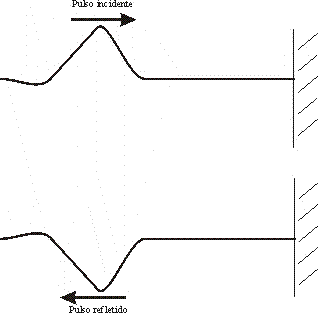
\includegraphics[width=0.6\textwidth]{refl1.png}
    \caption{Diagrama da reflexão de onda numa corda com a extremidade fixa. Perceba que a onda refletida é invertida em relação à onda incidente}
    \label{fig:reflexao_fixa}
\end{figure}

\subsection{Reflexão de ondas em cordas com extremidade presa a um suporte livre}

No caso da reflexão de uma onda se propagando por uma corda com a extremidade presa a um suporte livre, a onda refletida se mantém direita em relação à onda incidente.

\begin{figure}[H]
    \centering
    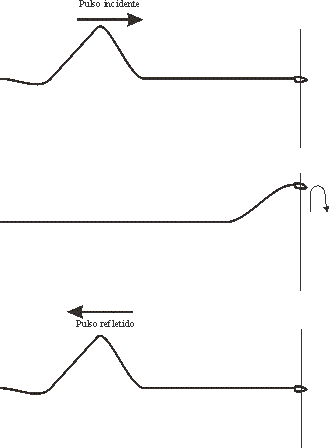
\includegraphics[width=.6\textwidth]{refl2.png}
    \caption{Diagrama de reflexão de onda numa corda com a extremidade presa a um suporte livre. Perceba que a onda refletida não é invertida na reflexão.}
    \label{fig:reflexao_livre}
\end{figure}

\section{Ondas Periódicas e Equação de Onda}
O tipo de onda mais conhecido e usado é o períodico, em que depois de um tempo $T$, a onda se repete.
A ilustração abaixo representa uma onda periódica:

\begin{figure}[H]
    \centering
    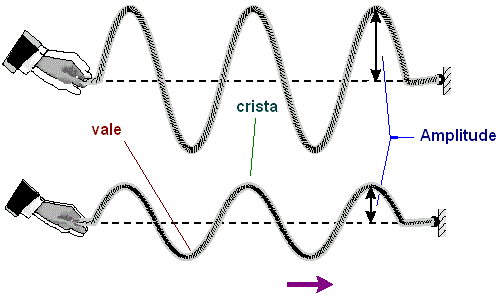
\includegraphics[width=0.6\textwidth]{periodicas.png}
    \caption{Representação de uma onda periódica. O ponto mais alto da onda é chamado de \textbf{crista}, enquanto o ponto mais baixo é chamado de vale. Uma onda maior significa que a sua amplitude aumentou}
    \label{fig:periodica}
\end{figure}
Com a crista e vale, pontos mais alto e baixo da onda, podemos definir uma quantidade da onda muito importante: \textbf{o comprimento de onda ($\lambda$).}

O comprimento de onda ($\lambda$) é a distância entre 2 cristas ou 2 vales consecutivos. Essa quantidade nos diz o tamanho que a onda tem antes que ela se repita. A unidade do comprimento de onda é metro (m)

A outra quantidade de interesse é \textbf{a frequência da onda ($f$)}. Ela nos diz por quantas repetições a onda passou em 1 segundo. A unidade da frequência é dada em Hertz ($Hz = 1/s$)

\begin{figure}[H]
    \centering
    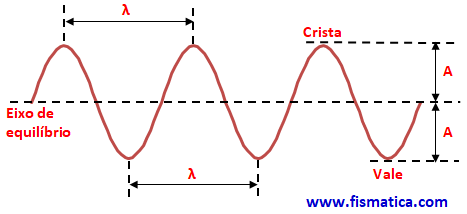
\includegraphics[width=0.6\textwidth]{lambda.png}
    \caption{Esquema mostrando o comprimento de onda, a onda e suas quantidades principais.}
    \label{fig:lambda}
\end{figure}

A principal relação que uma onda periódica possui é a chamada de \textbf{Equação de onda}:
\begin{equation}
    v=\lambda f
\end{equation}
\noindent em que $v$ é a velocidade da onda, $\lambda$ é o comprimento de onda e $f$ é a frequência da onda.

Perceba que para um mesmo meio, se aumentarmos a frequência da onda, por consequência, o comprimento de onda é menor. Isso traz implicações do tipo de onda para fenômenos que veremos nas próximas aulas, como difração e interferência.

Isso fica explícito no chamado \textbf{espectro eletromagnético da luz}:
\begin{figure}[H]
    \centering
    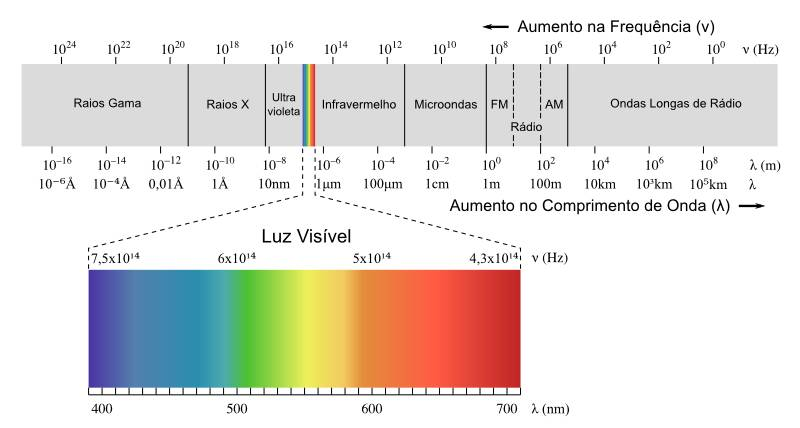
\includegraphics[width=0.9\textwidth]{espectro.jpg}
    \caption{Esquema do espectro eletromagnético da luz - perceba que o crescimento da frequência é para esquerda, enquanto o comprimento de onda cresce para a direita.}
    \label{fig:espectro}
\end{figure}

No espectro eletromagnético contém, basicamente, todos os tipos de luz que existem na natureza e, no caso da luz, a velocidade da onda é a velocidade da luz: $c=3.10^8\,m/s$. Já para ondas em cordas, a velocidade pode ser determinada por meio da equação (1).
\end{document}
